\documentclass[../../../../main.tex]{subfiles}
\begin{document}

\begin{flushright}
\footnotesize\textit{【自動文字起こし・要確認】}
\end{flushright}

[解]
(1) $f'(x) = 3x^2+2ax+b$ から、3次関数では接点と接線が一対一対応するので、$f'(x)=m$となる$x$の数にひとしい。\\
$f'(x)-m=0 \ \cdots$ \textcircled{1} の判別式$D$として
\begin{align*}
& \begin{cases}
D>0 \iff a^2-3(b-m)>0 & \text{の時 } 2\text{コ} \\
D=0 \iff a^2-3(b-m)=0 & \qquad 1\text{コ} \\
D<0 \iff a^2-3(b-m)<0 & \qquad 0\text{コ}
\end{cases} \quad \text{\#\ \ }
\end{align*}

(2) $P_1, P_2$の$x$座標 $\alpha, \beta$ とおく ($\alpha < \beta$としてよい)。と、これらは\textcircled{1}の2実数解である。\\
$l_1 : y=l_1(x), l_2 : y=l_2(x)$; $Q_1, Q_2$の$x$座標$q_1, q_2$として
\begin{align*}
f(x) - l_1(x) &= (x-\alpha)^2 (x-q_1) \quad \cdots \text{\textcircled{2}} \\
f(x) - l_2(x) &= (x-\beta)^2 (x-q_2) \quad \cdots \text{\textcircled{3}}
\end{align*}
$f(x)$は3次、$l_1(x), l_2(x)$は1次だから、2次の係数を比較して
\begin{align*}
& a = -2\alpha - q_1 = -2\beta - q_2 \\
& \text{（$a = -\frac{3}{2}(\alpha+\beta)$ だから辺々たして代入）} \\
& -3(\alpha+\beta) = -2(\alpha+\beta) - (q_1+q_2) \\
& \alpha+\beta = q_1+q_2 \\
& \therefore |\alpha-q_1| = |q_2-\beta|
\end{align*}
だから、$P_1, Q_1$の$x$座標の差と $P_2, Q_2$のそれが等しく、さらに$P_1Q_1, P_2Q_2$の傾きも等しいので、$\overline{P_1Q_1} = \overline{P_2Q_2}$ \quad $\blacksquare$

\vspace{1ex}
\noindent
[解2] [例の対称性を用いる]

$P_1(x_1, f(x_1)), P_2(x_2, f(x_2))$ の中点$M(p,q)$とすると
\begin{align*}
\begin{cases}
p = \frac{x_1+x_2}{2} \\
q = \frac{f(x_1)+f(x_2)}{2}
\end{cases}
\end{align*}
解と係数の関係から
\begin{align*}
q &= \frac{1}{2}(x_1^3+x_2^3) + \frac{a}{2}(x_1^2+x_2^2) + \frac{b}{2}(x_1+x_2) + c \\
&= \frac{2}{27}a^3 - \frac{ab}{3} + c \\
f(p) &= \left(\frac{x_1+x_2}{2}\right)^3 + \frac{a}{2}\left(\frac{x_1+x_2}{2}\right)^2 + b\left(\frac{x_1+x_2}{2}\right) + c = \frac{2}{27}a^3 - \frac{ab}{3} + c = q
\end{align*}
より、$M$は曲線上の点。次に$M$が原点になるように$f(x)$を平行移動すると
\begin{align*}
Y = X^3 + \left(b-\frac{a^2}{3}\right)X
\end{align*}
これは奇関数だから原点対称。よって$M$に関する対称性により$P_2, Q_2$を$P_1, Q_1$に重ねあわせることができるから\\
$\overline{P_1Q_1} = \overline{P_2Q_2}$ \quad $\blacksquare$

\begin{center}
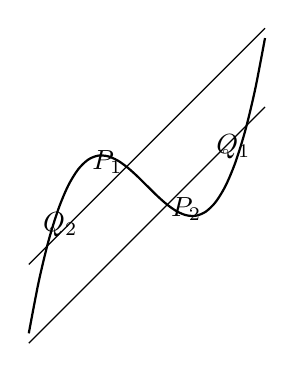
\begin{tikzpicture}
\draw[thick, domain=-1.5:1.5, smooth, variable=\x] plot ({\x}, {\x^3 - \x});
\node at (1.1, 0.5) {$Q_1$};
\node at (-1.1, -0.5) {$Q_2$};
\node at (-0.5, 0.3) {$P_1$};
\node at (0.5, -0.3) {$P_2$};
\draw (-1.5, -1) -- (1.5, 2);
\draw (-1.5, -2) -- (1.5, 1);
\end{tikzpicture}
\end{center}

\end{document}
